\section{Discussion}

Our updated modelling of MT provision in England has demonstrated that, as expected, the opening of more MT units improves outcomes for patients treated with MT. In our original 2020 report to NHS England \cite{allen2020}, we identified that the provision of 35--40 MT-capable centres represented a reasonable compromise between total admission numbers to CSCs whilst maintaining institutional competence in the procedure (at least 150 procedures per centre per year). We also identified those areas of England where the development of additional MT capacity would confer the greatest population benefit -- essentially areas that are both more populous and most distant from the existing MT provision in the 24 existing regional neurosciences centres, 6 of which are located in London. In descending order of population benefit, those locations were: Norfolk, East Kent, East Essex, the Somerset/Devon gap, Dorset coast, West Midlands, A1/M1 corridor north-west of London, and North East Manchester. Since 2020, additional MT capacity has been developed through new stand-alone thrombectomy centres at East Kent (opened 2026) and Norwich (due to open in 2027). Re-testing each current ASC as a single additional MT unit in this update (Table~\ref{tab:hospital-benefit}) shows that most of these areas remain among those with the greatest potential benefit -- the A1/M1 corridor north-west of London (Harrow and Watford, ranked first and third), the West Midlands (Smethwick, second), Greater Manchester (Stockport, fourth; Bury, 14th), the Dorset coast (Bournemouth, fifth) and the Somerset/Devon gap (Taunton, seventh) -- although their order has changed, East Essex (Colchester) now ranks 21st, and Worcester ranks 35th. The introduction of new stand-alone CSCs increases the total population benefit towards the maximum potential benefit were all acute stroke sites capable of delivering thrombectomy (Figure~\ref{fig:centres}, reproduced from Figure 11 of the 2020 report).

\begin{figure}[H]
\centering
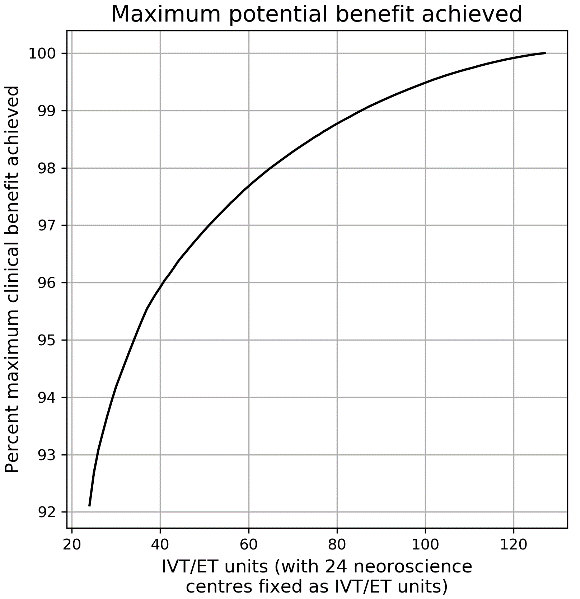
\includegraphics[width=0.5\linewidth]{images/centres.png}
\caption{Percentage of the maximum potential clinical benefit achieved as the number of MT-capable units increases, with the 24 neuroscience centres fixed as MT-capable units. Reproduced from Figure 11 of our 2020 report \cite{allen2020} (ET: endovascular thrombectomy).}
\label{fig:centres}
\end{figure}

This 2026 update to the national modelling confirms that this remains the case, although the increment in overall benefit to the English population is small -- two new centres increase the proportion of all stroke admissions that are admitted directly to a CSC from 33\% to 35\%, and the absolute increase in the proportion of patients with LVO with a `good outcome' (mRS 0--2 at 3--6 months, equivalent to independence in daily activities) rises from 12.4 to 12.6 percentage points. The impact on inequity is greater, in that two populous areas that currently have relatively remote access to MT through secondary transfer to a distant CSC gain a significant reduction in time to treatment, with a corresponding increase in the disability benefit for their local catchment population. In the case of Taunton (in the Somerset/Devon gap) and Worcester (to the south-west of Birmingham), this amounts to an absolute increase in the proportion of local patients treated with MT with a good outcome of 7.1 and 5.6 percentage points respectively.

However, any disability benefit accruing from new MT capacity is unequally distributed within the proposed two new regional networks, due to two factors which are already apparent within existing MT networks. The first is that the new MT capacity often yields only a relatively modest reduction in onset-to-treatment times for patients attending adjacent ASCs, who still require secondary transfer with all its attendant delays. A new MT centre in Taunton, for example, would become the closest CSC (in terms of travel time) for patients first attending the ASC in Dorchester, drawing in around 70 MT cases per year that are currently referred only a little further to Southampton. The reduction in onset-to-treatment time for these patients is small, and yields only a marginal 0.06 percentage point increase in the proportion of MT-treated patients with a good outcome. The effect for other adjacent ASCs is also modest (e.g.\ a new CSC at Worcester Royal Hospital would be only 15 minutes closer to Cheltenham than their current CSC in Bristol), yielding only an approximate 1 percentage point absolute increase in good outcomes. These more modest benefits are compounded by the second factor -- the observation that currently patients presenting first to an ASC have a 33\% lower likelihood of receiving MT when compared to apparently identical patients who present first at the doors of a CSC. This attrition is considered to be due to a number of factors linked to the fact that the patient is `elsewhere', but suggests that CSCs are operating a higher threshold of acceptance for MT for patients in an adjacent ASC than they operate for patients presenting directly to their own local service. This 33\% `referral attrition' would, presumably, be removed once a centre converts from an ASC to a CSC, but would persist for the remaining adjacent ASCs within the new networks -- with the effect of widening the difference in benefit between the two types of acute site. When taking account of this real-world effect, the absolute benefit from new MT capacity in Taunton would rise from 7.1 to 8.1 percentage points, whereas that for patients presenting first to Barnstaple would fall from 1.43 to 0.96 percentage points.

Despite these structural inequities, this updated modelling does serve to emphasise what we know from the research literature -- that there remains considerable additional population benefit from achieving substantial reductions in onset-to-treatment time for this most disabling type of stroke. This is most evident for the local catchments served by any new MT-capable centre, who lose the 113-minute delay that currently characterises patients requiring secondary transfer. Any measure, broadly applied, that reduces this delay will yield tangible disability benefits for all transferred patients. This might include measures to dramatically reduce door-in-door-out times at ASCs (currently running at just over 2 hours, compared with the 90 minutes assumed in our model), the selective pre-hospital identification of potential LVO patients for preferential bypass such as is currently being tested in the SPEEDY randomised trial \cite{shaw2026speedy}, or a more general permission for ambulance personnel to divert to a CSC if it is only 10--15 minutes further travel time. A 10-minute travel bias, if universally applied, would increase the population benefit from MT (the absolute increase in the proportion of LVO patients with a good outcome) from 12.6 to 13.7 percentage points (14.2 with a 15-minute bias), with the corollary that the proportion of all stroke admissions conveyed directly to a CSC would rise from 35\% to 57\% (69\% with a 15-minute bias) -- a 63\% relative increase in the number of patients admitted directly to CSCs (97\% with a 15-minute bias). This may be regarded as impractical or unsustainable for CSCs, but it serves to illustrate the general principle that a `mothership' system of bypassing ASCs for direct CSC admission, or any partial move towards this, is always likely to dominate over a `drip-and-ship' system in terms of population benefit from reperfusion. Put another way, it would suggest that the principal function of retaining ASCs is not so much to deliver reperfusion treatment more rapidly by reducing travel times, but instead to mitigate the very large and unsustainable numbers of direct admissions to CSCs that would otherwise occur under a `pure' mothership system.

This update to our 2020 analysis and report was specifically tasked with estimating the impact of potential new stand-alone MT capability at the existing ASCs in Taunton (Musgrove Park Hospital) and Worcester (Worcester Royal Hospital). These new sites would draw in MT activity from Barnstaple, Exeter and Dorchester to Taunton, and from Hereford and Cheltenham to Worcester, forming new regional MT networks. In addition, a very small number of patients (about 0.5 MT admissions per year) who would currently attend Dudley first would instead go directly to Worcester. Predicted MT procedure activity in Taunton (based on the assumption of 10\% MT eligibility at all referring sites) would be 272/year, procedures currently performed at Plymouth, Southampton or North Bristol. Although the additional benefit to patients from Dorset/south Somerset first attending the ASC in Dorchester (Dorset County Hospital) is only marginal, diversion of this activity to Taunton does not jeopardise institutional competence at Southampton, which remains a busy CSC. However, if Taunton were not to draw in this activity from Dorset, that may approach what is considered the lower limit of activity to maintain institutional competence (150 procedures/year, or 30 procedures/year for five operators), especially if the 33\% referral attrition from the three adjacent ASCs cannot be eradicated. In other words, despite its marginal position, Taunton needs to include Dorchester in order to sustain an appropriate level of MT activity. This dependency on adjacent ASCs is even more pronounced for a new CSC in Worcester, with approximately 80 of their predicted 202 MTs originating from Cheltenham. Any proposal to stage the introduction of MT at Worcester by limiting its initial catchment to only Hereford and Worcester would yield insufficient numbers of procedures to establish institutional competence -- an effect more pronounced if 33\% referral attrition from Hereford were to persist (in fact Hereford's MT rate for 2025/26 was 1.9\%). The impact on MT activity at the Queen Elizabeth Hospital in Birmingham would not be detrimental, in that it would remain a busy centre serving the West Midlands and the Black Country, but North Bristol would lose activity from both Cheltenham and Taunton, with 174 procedures delivered elsewhere and annual activity (for English patients) predicted to be 220 procedures/year. These activity figures assume that 10\% of all stroke patients receive MT. With the observed 33\% loss of MT for patients first attending an ASC, predicted activity falls to 214 procedures/year at Taunton and 159 at Worcester (Table~\ref{tab:mt_units_all}), and at the current national MT rate of 4.8\% activity at both new centres would be roughly half the modelled figures -- below the 150 procedures/year threshold. Clearly, as indications for MT continue to extend towards 12--15\% of all strokes \cite{mcmeekin2024}, these reductions in MT activity are much less likely to jeopardise institutional competence at any of the CSCs involved in the region, but at current rates of growth in MT activity (only a 10\% relative increase in each of the three years from 2023/24 to 2025/26), levels of 12--15\% are unlikely to be achieved for many years.

\subsection{Limitations}

The following limitations of this work should be considered.

\begin{itemize}

    \item In order to isolate the effect of geographic changes in provision of MT, we exclude non-geographic sources of variation from the model. For example, we assume that all MT units have the same use and speed of MT, meaning that the benefit of MT is dependent only on the time from onset to arrival at any given CSC. We, likewise, assume that the use and speed of IVT is unchanged by any changes to unit designation. We have drawn attention to the observation that, at present, MT rates for patients presenting first to an ASC are consistently lower than those seen for patients directly admitted to a CSC. This observation, and that which shows that onset-to-arrival times and door-in-door-out times are both significantly higher than the figures used in the optimised system we have modelled, will mean that the `real world' population benefit from reperfusion is at present significantly lower than that reported here.

    \item We assume that patients will attend their closest stroke unit (ASC or CSC) first (unless a travel bias is applied), and will then be transferred to the closest CSC, if required. Where differences in distances to alternative units are not very large, local arrangements or ambulance boundaries may mean that patients do not necessarily attend closest units. Usually we would expect this to only occur when differences in travel times are small, and so clinical benefit of IVT and MT should be substantially unchanged, but local arrangements may cause differences in the number of admissions an ASC or CSC would receive. Such arrangements, where they occur in the real world, will be reflected in the updated data for ASC admissions from SSNAP that we have used.

    \item The estimated benefit of IVT and MT is modelled here on clinical trial data which reports expected population average treatment effects depending on time to treatment. Our other work has demonstrated how treatment effects can vary depending on patient characteristics \cite{pearn2026machine}.
\end{itemize}

\section{Conclusions}

In this 2026 update to our original 2020 report `Maximising the Population Benefit from Reperfusion for Acute Ischaemic Stroke in England' \cite{allen2020}, we report the following conclusions:

\begin{enumerate}
    \item Expanding the number of thrombectomy-capable centres in England provides small incremental benefits in population disability for the nation as a whole, but addresses geographical inequity of access when additional capacity is developed in populous areas presently served by a distant CSC;
    \item The areas of greatest population benefit from developing new sites identified in 2020 remain broadly the same (Table~\ref{tab:hospital-benefit}), although their order has changed; in reality the sequence of developing MT capacity at new sites may be dictated by other considerations such as institutional readiness and workforce availability, rather than exclusively by predictions of population benefit;
    \item The modelling reported here highlights the regional inequities inevitable in a system dependent on secondary transfer for a time-sensitive, disability-reducing treatment. In the absence of the resources to develop MT capability in all acute stroke sites, these inequities can be mitigated by other measures aimed at reducing onset-to-treatment times (such as dramatically reducing door-in-door-out times at referring ASCs, or some form of preferential diversion of selected stroke patients for bypass directly to a CSC) and at eradicating the current 33\% reduction in the likelihood of MT treatment for eligible patients presenting first to an ASC;
    \item Specifically in relation to potential new MT capability in Taunton and Worcester, a centre (either in Exeter or Taunton) to fill the `Somerset/Devon gap' is high on the list of population gains, with tolerable reductions in activity at North Bristol and Plymouth. A centre to the south-west of Birmingham is less remote from existing provision, with a smaller catchment that is dependent on re-routing activity from Cheltenham. Particularly considering the 33\% `referral attrition' evident in the current system, a new site at Worcester would be more vulnerable at the lower limit of the activity considered necessary to maintain institutional competence.
\end{enumerate}
